% ------ headers globales y begin ---------------
\documentclass[11pt, a4paper, twoside]{article}
\usepackage{header_tp1}
\begin{document}{}
% -----------------------------------------------

\subsubsection{Descripción}

La optimización es una constante. Los escenarios anteriores buscaban optimizar
el tiempo de respuesta del algoritmo que solucione el problema. En este caso,
además de mantener la complejidad bajo cotas aceptables, es necesario optimizar
la solución del problema. Queremos que nuestro algoritmo lo resuelva en un
tiempo decente, pero la prioridad viene dada porque la resolución sea eficiente
en cuanto a las demandas solicitadas. Hay que cuidar un museo, cuyo objetos
son de gran valor. En estos casos podemos aceptar tardar un poco más siempre
que aseguremos que la solución es efectivamente la que minimiza el problema.

Cada piso del museo se puede modelar como una matriz de $n \times m$, dónde
cada elemento representa una porción equitativa y además contiene una propiedad.
Llamaremos $grilla$ a la matriz que modela el piso y $casilla$ a cada elemento
de la grilla. A priori, una celda puede estar libre, puede tener una pared
o puede tener una $reliquia$. Nuestro trabajo es cuidar las reliquias.
Para ello vamos a instalar sensores láser de modo tal que todas las celdas
que no son una pared tengan protección. Contamos con dos lásers, bi-direccionales
y cuatri-direccionales. Los \enquote{bi} sólo cubren en forma vertical u horizontal
y los \enquote{cuatri} en ambos sentidos. La celda libre en dónde se instala alguno
de los láser queda automáticamente protegida. Además, el rayo emitido desde el láser
protege toda su fila y/o columna hasta que se encuentra con una pared. Toda celda
libre que no tenga sensor láser debe tener al menos un rayo láser. Las reliquias
deben ser protegidas con exactamente dos rayos láser, siempre y cuando éstos
provengan uno desde una \enquote{fila} y el otro desde una \enquote{columna}.
No se pueden instalar sensores en la misma fila o columna salvo que una pared
se interponga entre ellos. Toda celda debe quedar cubierta o bien por 
una pared (de las existentes, no se pueden agregar) o bien por detección láser (sensor, rayo, doble rayo).

\begin{center}
\begin{figure}[H]
   \begin{center}
   \includegraphics[width=.9\textwidth]{img/descrip_ej3.png}
   \caption{\textbf{Una instancia del Problema 3 y dos soluciones distintas}}
   \label{fig:ej3-descrip}
   \end{center}
\end{figure}
\end{center}

El algoritmo debe realizar una ejecución con la técnica de \textit{backtracking}
devolviendo sólo la solución óptima (o alguna de ellas) en caso de existir.
O sea, en cada momento se preserva sólo la solución óptima parcial y se descartan las demás.
Esto tiene como provechoso el hecho de que al necesitar gastar la menor cantidad de dinero, si en medio
de una rama de posible solución ya superamos en costo a la posible solución óptima parcial guardada,
entonces podemos \textit{podar} esta rama desde la bifurcación próxima anterior sin necesidad
de completarla. De todas formas no se puede garantizar que se encuentre una solución.
Pero si existe, vamos a demotrar que es óptima.

\subsubsection{Hipótesis de resolución}

Para que podamos asegurar el museo, se reciben las dimensiones del piso ($n, m$) y su matriz asociada, donde
cada celda (o elemento) representa $1m^2$ del piso. Al momento de recibir la grilla, cada celda puede tener
sólo uno de los siguientes estados: \textsc{Pared}, \textsc{Libre}, \textsc{Reliquia}. Para diferenciarlos,
la cátedra asigna un valor a cada estado inicial, siendo $0, 1, 2$ respectivamente.

Toda celda con estado \textsc{Libre} o con una reliquia debe quedar protegida,
ya sea colocando un sensor sobre la misma o que el haz de láser emitido por un
sensor cruce la celda. Una solución al problema va tener uno y solo uno
de los siguientes estados: \textsc{SensorH}, \textsc{SensorV}, \textsc{SensorC},
\textsc{LaserH}, \textsc{LaserV} y \textsc{LaserC}.
En la siguiente tabla se describen cada uno de los estados:

\begin{center}
	\begin{tabular}{ l p{8cm} }
		\textbf{Estado celda} & \textbf{Descripción estado} \\
		\hline
		\textsc{SensorH} & En la celda hay un sensor bi-direccional que emite un haz de láser a lo largo de la fila.\\
		\textsc{SensorV} & En la celda hay un sensor bi-direccional que emite un haz de láser a lo largo de la columna.\\
		\textsc{SensorC} & En la celda hay un sensor cuatri-direccional que emite haz de láser a lo largo de la fila y otro a lo largo de la columna de la celda.\\
		\textsc{LaserH}  & La celda esta protegida por un haz de láser horizontal emitido desde otra celda de la fila.\\
		\textsc{LaserV}  & La celda esta protegida por un haz de láser horizontal emitido desde otra celda de la columna.\\
		\textsc{LaserC}  & La celda esta protegida por dos haces de láser, uno horizontal emitido por un sensor en la fila y otro vertical emitido por un sensor en la columna.
	\end{tabular}
\end{center}

El enunciado pide que las celdas que contengan reliquias estén protegidas por 2 haces de láser.
Luego, toda solución válida va tener el estado \textsc{LaserC} en las celdas que inicialmente
tenían el estado \textsc{Reliquia}.
Ésta es la primer cota que podemos aplicar a fin de reducir el procesamiento.

Dada una fila o columna, las celdas que las componen no pueden tener una
combinación arbitraria de los estados mencionados.
Por ejemplo, una fila no puede tener dos celdas con el estado \textsc{SensorH}.
Este tipo de restricción impuesta por el enunciado nos permite aplicar podas,
dado que sabemos a priori que ciertas combinaciones de estados son imposibles.

En la siguiente tabla se muestran que combinaciones de estados son posibles en las filas y columnas de la grilla.
\begin{table}
\begin{center}
	\begin{tabular}{ | l | p{5cm} |p{5cm} | }
		\hline
		\textbf{Estado celda} & \textbf{Fila puede contener celdas con estado} & \textbf{Columna puede contener celdas con estado} \\
		\hline
		\textsc{SensorH} & \textsc{LaserC}, \textsc{LaserH} & \textsc{LaserH}, \textsc{SensorH} \\		\hline
		\textsc{SensorV} & \textsc{LaserV}, \textsc{SensorV} & \textsc{LaserV}, \textsc{LaserC}\\ 		\hline
		\textsc{SensorC} & \textsc{LaserC}, \textsc{LaserH} & \textsc{LaserC}, \textsc{LaserV}\\ 		\hline
		\textsc{LaserH}  & \textsc{LaserC}, \textsc{LaserC}, \textsc{SensorC}, \textsc{LaserH}, \textsc{SensorH} &  \textsc{LaserH}, \textsc{SensorH} \\ 		\hline
		\textsc{LaserC}  & \textsc{LaserC}, \textsc{LaserC}, \textsc{SensorC}, \textsc{LaserH}, \textsc{SensorH} & \textsc{LaserC}, \textsc{SensorC}, \textsc{LaserV}, \textsc{SensorV} \\ 		\hline
		\textsc{LaserV}  & \textsc{LaserV}, \textsc{SensorV} & \textsc{LaserC}, \textsc{SensorC}, \textsc{LaserV}, \textsc{SensorV}  \\ \hline
	\end{tabular}
	
\end{center}
\caption{Combinaciones posibles de estados}
		\label{tab:Estados}
\end{table}

Los estados válidos para una celda van a estar dados por la intersección
entre los estados posibles de la fila y la columna a la que cada celda pertenezca.
La información contenida en la tabla no es suficiente para podar correctamente.
Por ejemplo, si nos basamos sólo en esta tabla podríamos tomar como solución una grilla
donde una columna en la cual todas sus celdas se encuentren en el estado \textsc{LaserV}.
Esta solución es incorrecta dado que no hay sensor que emita el haz de láser,
contradiciendo lo descripto en la tabla de estados. Esto nos permite aplicar otra poda.
Al saber de antemano que toda fila en la cual alguna de sus celdas tiene el estado \textsc{LaserC} o \textsc{LaserH},
se requiere que alguna celda dentro de la fila se encuentre en estado \textsc{SensorC} o \textsc{LaserH}.
Análogamente para las columnas, cuando alguna de sus celdas tiene el estado \textsc{LaserC} o \textsc{LaserV}
se requiere que una celda dentro de la columna tenga el estado \textsc{SensorC} o \textsc{LaserV}.

Por el momento, en todo lo analizado previamente no se tuvo en cuenta las celdas con estado inicial \textsc{Pared}.

\begin{figure}[H]
	\begin{center}
		\begin{tabular}{ | l | l | l | l | l | }
			\hline 
			&$ $ & \cellcolor{black}&  &\\ \hline 
			& & &  &\\ \hline 
			\cellcolor{black}& &\cellcolor{black} &  &\cellcolor{black} \\ \hline 
			& & &  &\\ \hline 
		\end{tabular}
		\caption{Dibujo de grilla con paredes}
		\label{fig:grilla-pared}
	\end{center}
\end{figure}

Por ejemplo, en grilla de la ~\fig{fig:grilla-pared} se puede ver que la primer fila
se encuentra dividida en 2 por una pared, lo cual nos da 2 sub-filas totalmente independientes entre sí.
Con esto queremos decir que la selección de estado de las celdas de la sub-fila 1 no implica
una reducción en los posibles estados que puedan tomar las celdas de la sub-fila 2.
En este caso las podas pensadas anteriormente pierden cierta efectividad.
%Habria que analizar como afecta la poda la pared

Luego, en la tercer fila se puede ver la misma situación con la particularidad
que la longitud de una de las sub-filas es de 1 celda. Es evidente que dicha celda 
no va poder tomar ningún estado que implique que hay un haz de láser horizontal sobre la celda,
o sea los estados \textsc{LaserC} y \textsc{LaserV}, dado que no hay celda en dicha sub-fila que emita el haz.
Detectar sub-filas y sub-columnas de longitud 1 nos permitirá probar en dichas celdas solo los casos posibles y correctos.

Es posible que algunas grillas no admitan solución. Por ejemplo una grilla que 
contenga toda un fila/columna (o sub-fila/columna) donde todas las celdas que la 
componen tengan como estado inicial \textsc{Reliquia}. Una situación parecida se 
presenta a cuando una sub-fila/columna de 1 celda contiene una celda con 
estado inicial \textsc{Reliquia}. Es importante poder detectar este tipo 
de situación lo antes posible y evitar malgastar tiempo de cómputo.

La primer táctica de solución que se consideró para resolver el problema
consistía en modificar el estado de las celdas con estado inicial \textsc{Libre}
por los diferentes estados de sensor. Luego modificar las celdas de fila y/o 
columna sobre las cuales proyectara el sensor en cuestión, con el estado de haz emitido
por él mismo. Luego escanear la grilla a fin de validar que cumple que dicha 
solución parcial cumpliera con los requerimientos. De cumplir con los requerimientos 
se procedería a completa la próxima celda con estado \textsc{Libre}, nuevamente 
con los diferentes sensores y se repetiría el mismo procedimiento hasta que no haya
celdas con estado inicial \textsc{Libre}. De no cumplir con los requerimientos 
se volvería al estado anterior, para luego probar con otro tipo de sensor.
Esta táctica, a pesar de ser correcta, requería escanear la grilla cada
vez que se probaba un nuevo estado en una celda, lo cual resultaba
computacionalmente costoso, por lo cual decidimos buscar otra alternativa de solución.

La segunda táctica que se consideró, que fue la que finalmente utilizamos,
consiste en tener en todo momento conocimiento de los estados posibles 
que pudiesen tener celdas de la grilla. La grilla se completa en orden,
de a 1 celda \textsc{Libre} a la vez, modificando los estados disponibles 
para  la fila/columna  de la celda según las especificaciones de la tabla ~\ref{tab:Estados}.
A diferencia de la táctica anterior, no solo completamos las celdas con sensores,
también es posible completar una celda con alguno de los estados de láser.
De llegar a procesar todas las celdas con estado \textsc{Libre} sabremos que dicha 
solución cumple con los requerimientos del problema, dado que se completó
aplicando las restricciones solicitadas por el enunciado.

En el caso que la solución parcial no llegue a ser una solución, eventualmente
se llegará a procesar alguna celda para la cual no hay estados posibles,
con lo cual se deberá retroceder a las celdas previas y continuar probando
con combinaciones de estados diferentes. Esta táctica nos permite evitar 
escanear la grilla cada vez que se modifica el estado de la grilla, 
aunque requiere mayor consumo de memoria. 

Las opciones de las celdas se calcularán haciendo una intersección entre los estados
disponibles de la fila y columna de cada celda. Se guardan y se mantendrán actualizados
los estados posibles de cada fila/columna de la grilla, los mismos estarán 
codificados en una máscara según se muestra en la \fig{fig:mascaraEstados}.

\begin{figure}[H]
\begin{center}
	\begin{tabular}{ | l | l | l | l | l | l | l | l | }
		\hline 
		Req	& LV & LH & LC & SV & SH & SC  & 0\\
		\hline 		
	\end{tabular}
\end{center}
\caption{Mascara de estados disponibles para columna/fila}
\label{fig:mascaraEstados}
\end{figure}

El primer bit comenzando desde la derecha no se utiliza y siempre se mantiene en 0.
Los 6 campos siguientes, de tamaño de 1 bit, toman el valor 1 cuando el estado
está permitido para la celda/columna y 0 cuando no.

\begin{center}
\begin{tabular}{ r | l }
	SC & Estado \textsc{SensorC} \\
	SH & Estado \textsc{SensorH} \\
	SV & Estado \textsc{SensorV} \\
	LC & Estado \textsc{LaserC}  \\
	LH & Estado \textsc{LaserH}  \\
	LV & Estado \textsc{LaserV}  \\
	Req & Estado Requerimiento Fila/Columna (2 bits) \\
			& \hspace{.5cm}{\small \textrm{Puede tomar los siguientes valores}} \\
		  & \hspace{.8cm}{\small \textrm{00 - No Requiere Sensor}} \\
		  & \hspace{.8cm}{\small \textrm{01 - Requiere Sensor}} \\
		  & \hspace{.8cm}{\small \textrm{02 - Tiene Sensor}}
\end{tabular}
\end{center}

Como se mencionó antes, una celda con estado \textit{Pared} genera múltiples
sub-filas/columnas independientes, por lo que será necesario guardar el cambio de estado que implica cada pared.

Primero se analizará la grilla, generando las opciones iniciales para cada fila/columna.
De detectar que el problema no tiene solución se terminará la ejecución inmediatamente.
Luego, dentro del espectro de soluciones posibles resultantes de este análisis
probaremos todas las combinaciones de estados, quedándonos con la solución de menor costo.
A fin de mejorar el tiempo de ejecución se agrega una poda más, que consiste en dejar
de procesar toda solución parcial que sea mayor o igual a la mejor solución que se haya encontrado hasta el momento. 
En el \alg{secmuseo} se puede observar lo descripto.

\begin{algorithm}
\caption{Asegurar Museo}\label{secmuseo}
\begin{algorithmic}[1]
	\Require
		\Statex $n, m \gets$ \Call{Int}{} \Comment{dimensiones de la matriz}
		\Statex $G \gets$ \Call{Matriz de $n \times m$}{} \Comment{grilla de celdas}
	\Ensure
		\Statex \Call{Cantidad de Sensores}{} \Comment{si es $-1$, no existe solución}
		\Statex \Call{Costo de la Solución}{}
		\Statex \Call{Lista de Sensores}{} \Comment{$sensor = (tipo, fila, columna)$}
	\Statex{}
	
	\State $opcionesFilas \gets $ \Call{Nuevo Vector}{$n$} \Comment{posibilidades en cada celda}
	\State $opcionesCol \gets $ \Call{Nuevo Vector}{$m$}
	\State $opciones \gets $ \Call{Nuevo Par}{$opcionesFilas,opcionesCol$}
	\State $celdasProcesar \gets$ \Call{Nueva Lista}{}
	\State $solucion \gets$ \Call{Nueva Lista de Sensores}{}
	\State $solucionOptima \gets$ \Call{Nueva Lista de Sensores}{}
	\Statex
	
	\State \Call{cargar}{$n, m, G$}
	\If { \Call{Analizar}{$G,opciones,celdasPocesar$} $=$ \Call{Tiene Solución}{} } \Comment{ \bigO{n}}
		\State \Call{backtrack}{$G, opciones, celdasPocesar, solucion, solucionOptima$} \Comment{ \bigO{n*6^n}}
		\State \Return $solucion$
	\EndIf
	\Statex
	
	\Function {Analizar}{$G, opciones, celdasPocesar$}
		\State $FilaValida \gets $ \Call{Nuevo Vector}{$n$} \Comment{Máscaras que verifican validez de filas}
		\State $ColValida \gets $ \Call{Nuevo Vector}{$m$} \Comment{Máscaras que verificar validez de columnas}
		\State $opcionesFilas \gets $ \Call{Primero}{$opciones$}
		\State $opcionesCol \gets $ \Call{Segundo}{$opciones$}
		
		\ForTo {$i$}{$1$}{$n$}
			\ForTo {$j$}{$1$}{$m$}
				\State \Call{OR Binario}{$FilaValida[i],G[i][j]$}
				\State \Call{OR Binario}{$ColValida[i],G[i][j]$}
				\State $mascara \gets $\Call{AnalizarCelda}{$G, i, j, celdasProcesar$}
				\If {$mascara$ \Is \Call{Configuración Invalida}{}}
					\State \Return \Call{No Tiene Solución}{}
				\EndIf
				\State \Call{Actualizar Opciones Fila}{$opcionesFila, i, mascara$}
				\Statex \Comment{Actualiza opciones Fila o asigna opciones a Pared}
				\State \Call{Actualizar Opciones Columna}{$opcionesCol, j, mascara$}
				\Statex \Comment{Actualiza opciones Columna o asigna opciones a Pared}
			\EndFor
		\EndFor
		\ForTo {$i$}{$1$}{$n$}
			\If{$FilaValida[i]$ \Is \Call{Fila Invalida}{}}
				\State \Return \Call{No Tiene Solución}{}
			\EndIf
		\EndFor
		
		\ForTo {$j$}{$1$}{$m$}
			\If{$ColValida[j]$ \Is \Call{Col Invalida}{}}
				\State \Return \Call{No Tiene Solución}{}
			\EndIf
		\EndFor
		\State \Return \Call{Tiene Solución}{}
	\EndFunction
	\algstore{bkbreak}
\end{algorithmic}
\end{algorithm}

\clearpage
\begin{algorithm}[h!]
\caption{Asegurar Museo (continuación)}
\begin{algorithmic}[1]
	\algrestore{bkbreak}
	
	\Procedure {Backtrack}{$G, opciones, celdasPocesar, solucion, solucionOptima$}
		\State $snapshot \gets $\Call{Nueva Tupla}{$Vector, Vector, Opcion$}
		\State $opcionesFilas \gets $ \Call{Primero}{$opciones$} 
		\State $opcionesCol \gets $ \Call{Segundo}{$opciones$} 
		\If {$celdasProcesar$ \Is \Call{Vacio}{}}
			\State $celda \gets $ \Call{Obtener Primer Elemento}{$celdasProcesar$}	
			\State $mascaraFila \gets $ \Call{Obtener Mascara Fila}{$celda,opcionesFilas$} 
			\State $mascaraColumna \gets $ \Call{Obtener Mascara Columna}{$celda, opcionesCol$} 
			\State $mascaraRequerimiento \gets$ \Call{Requiere Sensor}{$mascaraFila, mascaraColumna, celda$} 
			\State $mascaraCelda \gets $\Call{AND Binario}{$mascaraFila, mascaraColumna, mascaraRequerimiento$} 
			\State $snapshot \gets $ \Call{Guardar Estado}{$opcionesFilas, opcionesCol, celda$} 
			\ForAll{$opcion$ \textbf{en} \Call{Opciones}{}}
				\State $opValida \gets$ \Call{Es Valida}{$mascaraCelda, opcion$} 
				\State $precioOp \gets$ \Call{Precio}{$opcion$} 
				\State $precioSol \gets$ \Call{Precio}{$solucion$} 
				\State $precioSolOptima \gets$ \Call{Precio}{$solucionOptima$} 
				\If {$ opValida \wedge (precioSol + precioOp < precioSolOptima)$}
						\State \Call{Actualizar Estado}{$opcion, opcionesFilas, opcionesCol$} 
						\State \Call{Backtrack}{$G, opciones, celdasPocesar, solucion, solucionOptima$} 
						\State \Call{Actualizar Estado}{$snapshot, opcion, opcionesFilas, opcionesCol$} 
				\EndIf
			\EndFor
		\Else
			\If{\Call{Precio}{$solucion$} $<$ \Call{Precio}{$solucionOptima$}}
				\State $solucionOptima \gets solucion$ \Comment{\bigO{n}}
			\EndIf
		\EndIf
	\EndProcedure
	\Statex
	
	\Function {Analizar Celda}{$G, i, j, celdasProcesar$}
		\State $mascara \gets$  \Call{Configuración Inválida}{}
		\If {$celdasProcesar$ \Is \Call{Libre}{}}
			\State \Call{Agregar Al Final De Lista}{$libre$}
			\State $mascara \gets$ \Call{Mascara No Hay Cambios}{}
		\ElsIf {$celdasProcesar$ \Is \Call{Reliquia}{}}
			\State $G[i][j] \gets$ \Call{LaserC}{}
			\If {\Call{Esta Rodeada Por Paredes}{$G,i,j$} \Is \Call{Falso}{}}
				\State $mascara \gets$ \Call{Máscara Laser C}{}
			\EndIf
		\ElsIf {$celdasProcesar$ \Is \Call{Pared}{}}
			\State $mascaraFila \gets$ \Call{Generar Máscara Según Longitud Sub Fila}{$G,j$}
		 	\State $mascaraCol \gets$ \Call{Generar Máscara Según Longitud Sub Col}{$G,j$}
		 	\State $mascara \gets$ \Call{OR Binario}{$mascaraFila, mascaraCol$}
		\EndIf
		\State \Return $mascara$
	\EndFunction
	
\end{algorithmic}
\end{algorithm}

\clearpage
\subsubsection{Justificación formal de correctitud}

Como se describió en las secciones anteriores, en todo momento se tiene total
conocimiento de todos los estados posibles (y correctos) que puede tener cada celda.
Para ello se escanea la grilla a fin de recopilar las condiciones iniciales de la grilla. 
Al escanear la grilla también se verifica que la misma tenga solución,
en el caso de detectar que no tiene solución se interrumpe el algoritmo.
Cada vez que se \enquote{completa} una celda, se actualizan las opciones
disponibles para la fila y/o columna de la celda, asegurando que próximas
llamadas solo se utilizarán estados correctos. Esto, sumado se a que se modifica
el estado de las celdas de manera ordenada, nos permite asegurar que de llegar a una solución,
es decir, llegar a un estado donde no queden celdas con estado \textit{Libre},
la solución es válida. Antes de completar una celda con alguna de las opciones disponibles
se guarda el estado, esto permite que al retornar el procedimiento \textsc{Backtrack}
se restaure el estado previo para poder probar con el resto de la opciones. 
Toda nueva solución encontrada se compara contra la mejor solución encontrada hasta el momento.
De superarla, se guarda la nueva solución como óptima.
Esto nos asegura que al terminar el algoritmo, en caso de  encontrar una solución, será óptima. 

\subsubsection{Cota de complejidad temporal}

El \alg{secmuseo} consiste, en el caso de que la grilla tenga solución, en la ejecución secuencial de los procedimientos \textsc{Analizar Grilla} y \textsc{Bactrack}. 

Ambos procedimientos utilizan estructuras provistas por la biblioteca estándar de C++. Se utilizan vectores, std::vector , para guardar las mascaras de cada fila/columna,y para la grilla se utiliza un vector de vectores.  Por lo documentado en la biblioteca estándar de C++, std::vector nos garantiza  acceso aleatorio con orden constante.  Para almacenar la lista de celdas a procesar se utiliza std::list, sobre dicha estructura solo se realizan operaciones de inserción/borrado al inicio y final de la lista, siendo estas operaciones de orden constante según lo documentado en la biblioteca estándar de C++.


El procedimiento \textsc{Analizar Grilla} recorre la grilla actualizando
estados de celdas y modificando opciones de la fila y/o columna de la celda analizadas.
Las operaciones que se ejecutan por celda se pueden considerar constantes.
Al análisis de la grilla es \bigO{n}. Luego se recorren las opciones resultantes
de cada fila y columna para verificar la validez de la grilla, con una complejidad
\bigO{\#filas} y \bigO{\#columnas} respectivamente. El orden del procedimiento
será \bigO{\textsc{Máx}(n,\#fila,\#columna)}. Como $n$ es mayor que
$\#filas$ y $\#columnas$ para toda grilla, \textsc{Analizar Grilla} resulta \bigO{n}.

Ahora analizamos la complejidad de \textsc{Bactrack}. Sea $T(i)$ el tiempo que demora el procedimiento
\textsc{Bactrack} con un entrada de tamaño $i$. Para el caso donde $i = 0$,
se verifica si la solución encontrada y guardada en el vector $solucion$
tiene un costo menor que a la solución guardada. De tener un menor precio,
se copian los valores de la solución actual al vector $solucion\_optima$.{}
Guardar la nueva solución implica eliminar los $k$ elementos del vector $solucion\_optima${}
y luego hacer inserción de los $k'$ sensores de la nueva solución.
Por documentación de la biblioteca estándar de \texttt{C++}, sabemos que
en el peor de los casos la operación de borrar $k$ elementos es \bigO{k} \bib{stl:vector}.
La inserción de un elemento al final del vector es constante,
luego la inserción de $k'$ elementos $\in$ \bigO{k'}. Dado que no puede haber
más sensores que celdas, $k \leq n$ y $k' \leq n$, resultando \bigO{n} para el caso $i = 0$.
Para los casos $n \geq 1$, se harán en el peor de los casos con 6 llamadas recursivas
(una por cada opción disponible) de duración \bigT{n-1} cada una.
Considerando el resto de las operaciones, que consisten en comparaciones, sumas y
operaciones lógicas de enteros de 32 bits, de complejidad constante,
obtenemos la siguiente ecuación de recurrencia:

\begin{equation*}
	T(i) = \left\{
  \begin{array}{l l}
    n 					 & \quad \text{si } i = 0 \\
    6 * \bigT{i-1} & \quad \text{si } i > 1
  \end{array} \right.
\end{equation*}

Calculamos \bigT{n} para algunos valores de $n$:

\begin{align*}
	\bigT{0} &= n \\
	\bigT{1} &= 6 * \bigT{0} = n * 6 \\
	\bigT{2} &= 6 * \bigT{1} = 6 * 6 * \bigT{0} = n * 6^{2} \\
	\bigT{3} &= 6 * \bigT{2} = 6 * 6 * \bigT{1} = 6 * 6 * 6 * \bigT{0} = n * 6^{3} \\
\end{align*}

Se puede conjeturar de los casos anteriores que \bigT{i} $= n * 6^{i}$.
Probamos la conjetura utilizando inducción en $i$. 

\paragraph*{Caso Base} $i=0$. Por definición \bigT{0} $= k$. Luego, \bigT{0} $= n * 6^{0} = n * 1 = i$. Verdadero para el caso base.

\paragraph*{Paso Inductivo} HI: $\bigT{i} = n * 6^{i}$.
Queremos probar $\bigT{i} \then \bigT{i+1}$. 
\[
	T(i+1) = 6 * T(i) \underset{\text{HI}}{=} 6 * (n * 6^{i}) = n \cdot 6^{i+1}
\]
Con lo cual \bigT{i} vale $\forall \ i$. Entonces \bigT{i} $\in$ \bigO{n * 6^i}.
Para el caso de una grilla con $n$ celdas libres \bigT{n} $\in$ \bigO{n * 6^n}. $\qed$ \\

Como \textsc{Analizar Grilla} $\in$ \bigO{n}, \textsc{Bactrack} $\in$ \bigO{n * 6^n}
y además $\forall \ n, \; n * 6^n > n$, podemos concluir que \alg{secmuseo} $\in$ \bigO{n * 6^n}.

\subsubsection{Verificación mediante casos de prueba}

Para verificar el correcto funcionamiento del algoritmo se generaron grillas
pequeñas posicionando paredes en cada una de ellas de tal manera de probar
que cada una de las podas funcionasen correctamente y que no se llegue
a soluciones incorrectas. A continuación se listan las pruebas mas representativas.

\paragraph{Caso de Prueba 1}\mbox{}\\

\begin{verbatim}
Entrada      Salida
-------      ------
3 3          3 14000
1 1 1        3 1 2
1 2 2        3 1 3
1 1 1        1 2 1
\end{verbatim}

\begin{figure}[H]
	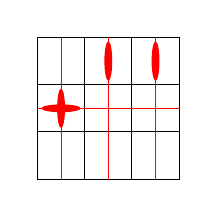
\begin{tikzpicture}[baseline=(current bounding box.north)]
	\matrix [minimum width=0.6cm ,minimum height=0.6cm,row sep=-\pgflinewidth,column sep=-\pgflinewidth ]
	{
	\node (11) [rectangle,draw] {}; & \node (12) [rectangle,draw]{};\fill[red] ellipse (0.05cm and 0.25cm); & \node (13) [rectangle,draw] {};\fill[red] ellipse (0.05cm and 0.25cm); \\
	\node (21) [rectangle,draw] {};\fill[red] ellipse (0.05cm and 0.25cm);\fill[red] ellipse (0.25cm and 0.05cm); & \node (22) [rectangle,draw] {$\blacklozenge$}; & \node (23) [rectangle,draw] {$\blacklozenge$}; \\
	\node (31) [rectangle,draw] {}; & \node (32) [rectangle,draw]{}; & \node (33) [rectangle,draw] {}; \\
	};
	\draw [-,red] (11.north) -- (31.south);
	\draw [-,red] (12.north) -- (32.south);
	\draw [-,red] (13.north) -- (33.south);
	\draw [-,red] (21.west) -- (23.east);
	\end{tikzpicture}
\end{figure}

\paragraph{Caso de Prueba 2}\mbox{}\\

\begin{verbatim}
Entrada      Salida
-------      ------
3 4          4 18000
1 2 2 1      1 1 1
1 1 1 1      3 2 2
1 1 0 1      3 2 3
             3 2 4
\end{verbatim}


\begin{figure}[H]
	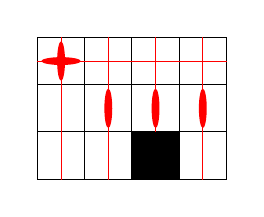
\begin{tikzpicture}
	\matrix [minimum width=0.6cm ,minimum height=0.6cm,row sep=-\pgflinewidth,column sep=-\pgflinewidth ]
	{
	\node (11) [rectangle,draw] {};\fill[red] ellipse (0.05cm and 0.25cm);\fill[red] ellipse (0.25cm and 0.05cm); & \node (12) [rectangle,draw]{$\blacklozenge$}; & \node (13) [rectangle,draw] {$\blacklozenge$};& \node (14) [rectangle,draw] {};\\
	\node (21)  [rectangle,draw] {}; & \node (22) [rectangle,draw] {};\fill[red] ellipse (0.05cm and 0.25cm); & \node (23) [rectangle,draw] {};\fill[red] ellipse (0.05cm and 0.25cm); & \node (24) [rectangle,draw] {};\fill[red] ellipse (0.05cm and 0.25cm);\\
	\node (31) [rectangle,draw] {}; & \node (32) [rectangle,draw]{}; & \node (33) [rectangle,draw,fill=black] {}; & \node (34) [rectangle,draw] {};\\
	};
	\draw [-,red] (11.north) -- (31.south);
	\draw [-,red] (11.west) -- (14.east);
	\draw [-,red] (12.north) -- (32.south);
	\draw [-,red] (13.north) -- (23.south);
	\draw [-,red] (14.north) -- (34.south);
	\end{tikzpicture}
\end{figure}

\paragraph{Caso de Prueba 3}\mbox{}\\

\begin{verbatim}
Entrada      Salida
-------      ------
3 5
0 1 2 1 0    4 18000
1 1 1 1 0    2 1 2
1 1 1 1 0    2 2 1
1 1 1 0 1    1 3 3
             2 3 5
\end{verbatim}

\begin{figure}[H]
	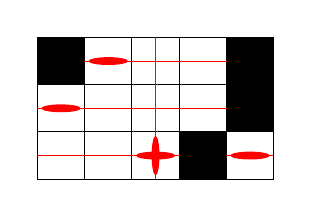
\begin{tikzpicture}
	\matrix [minimum width=0.6cm ,minimum height=0.6cm,row sep=0 ,column sep=0,row sep=-\pgflinewidth,column sep=-\pgflinewidth]
	{
	\node (11) [rectangle,draw,fill=black] {}; & \node (12) [rectangle,draw]{};\fill[red] ellipse (0.25cm and 0.05cm); & \node (13) [rectangle,draw] {$\blacklozenge$}; & \node (14) [rectangle,draw]{}; & \node (15)  [rectangle,draw,fill=black] {}; \\
	\node (21) [rectangle,draw] {};\fill[red] ellipse (0.25cm and 0.05cm); & \node (22) [rectangle,draw]{}; & \node (23) [rectangle,draw] {}; & \node (24) [rectangle,draw]{}; & \node (25) [rectangle,draw,fill=black] {}; \\
	\node (31) [rectangle,draw] {}; & \node (32) [rectangle,draw]{}; & \node (33) [rectangle,draw]{};\fill[red] ellipse (0.05cm and 0.25cm);\fill[red] ellipse (0.25cm and 0.05cm); & \node (34) [rectangle,draw,fill=black] {}; & \node (35) [rectangle,draw] {};\fill[red] ellipse (0.25cm and 0.05cm); \\
	};
	\draw [-,red] (12.west) -- (14.east);
	\draw [-,red] (21.west) -- (24.east);
	\draw [-,red] (13.north) -- (33.south);
	\draw [-,red] (31.west) -- (33.east);
	\draw [-,red] (35.west) -- (35.east);
	\end{tikzpicture}
\end{figure}

\paragraph{Caso de Prueba 4}\mbox{}\\

\begin{verbatim}
Entrada      Salida
-------      ------
5 5          8 32000
1 1 0 1 1    2 1 1
1 1 0 1 1    2 1 4
0 0 0 0 0    2 2 1
1 1 0 1 1    2 2 4
1 1 0 1 1    2 4 1
1 1 0 1 1    2 4 4
             2 5 1
             2 5 4
\end{verbatim}

\begin{figure}[H]
	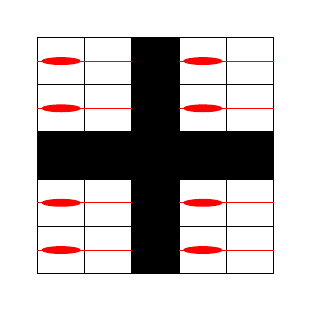
\begin{tikzpicture}
	\matrix [minimum width=0.6cm ,minimum height=0.6cm,row sep=0 ,column sep=0,row sep=-\pgflinewidth,column sep=-\pgflinewidth]
	{
	\node (11) [rectangle,draw] {};\fill[red] ellipse (0.25cm and 0.05cm); & \node (12) [rectangle,draw]{}; & \node (13) [rectangle,draw,fill=black] {}; & \node (14) [rectangle,draw] {};\fill[red] ellipse (0.25cm and 0.05cm);& \node (15) [rectangle,draw] {}; \\
	\node (21) [rectangle,draw] {};\fill[red] ellipse (0.25cm and 0.05cm); & \node (22) [rectangle,draw]{}; & \node (24) [rectangle,draw,fill=black] {}; & \node (24) [rectangle,draw] {};\fill[red] ellipse (0.25cm and 0.05cm); & \node (25) [rectangle,draw] {}; \\
	\node (31) [rectangle,draw,fill=black] {}; & \node(32) [rectangle,draw,fill=black]{}; & \node(33) [rectangle,draw,fill=black] {}; & \node(34) [rectangle,draw,fill=black] {}; & \node (31) [rectangle,draw,fill=black] {}; \\
	\node (41) [rectangle,draw] {};\fill[red] ellipse (0.25cm and 0.05cm); & \node (42) [rectangle,draw]{}; & \node (43) [rectangle,draw,fill=black] {}; & \node (44) [rectangle,draw] {};\fill[red] ellipse (0.25cm and 0.05cm); & \node (45) [rectangle,draw] {}; \\
	\node (51) [rectangle,draw] {};\fill[red] ellipse (0.25cm and 0.05cm); & \node (52) [rectangle,draw]{}; & \node (53) [rectangle,draw,fill=black] {}; & \node (54) [rectangle,draw] {};\fill[red] ellipse (0.25cm and 0.05cm); & \node (55) [rectangle,draw] {}; \\
	};
	\draw [-,red] (11.west) -- (12.east);
	\draw [-,red] (14.west) -- (15.east);
	\draw [-,red] (21.west) -- (22.east);
	\draw [-,red] (24.west) -- (25.east);
	\draw [-,red] (41.west) -- (42.east);
	\draw [-,red] (44.west) -- (45.east);
	\draw [-,red] (51.west) -- (52.east);
	\draw [-,red] (54.west) -- (55.east);
	\end{tikzpicture}
\end{figure}

\paragraph{Grillas sin solución}\mbox{}\\

Por último se probó el algoritmo en las siguientes grillas sin solución.
El algoritmo detectó la imposibilidad de resolver las grillas devolviendo
$-1$ como es requerido por el enunciado.

\begin{figure}[H]
	\begin{center}
	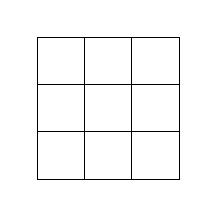
\begin{tikzpicture}
	%    \edef\gRows{#1}
	%    \edef\gCols{#2}
	%    \edef\gValues{#3}
	%    \edef\hsize{0.5cm}
	%[matrix minimum width=0.8cm,minimum height=0.8cm,row sep=0  ]

	\matrix [minimum width=0.6cm ,minimum height=0.6cm,row sep=0 ,column sep=0,row sep=-\pgflinewidth,column sep=-\pgflinewidth]
	{
	\node [rectangle,draw] {}; & \node[rectangle,draw]{}; & \node[rectangle,draw] {}; \\
	\node[rectangle,draw] {$\blacklozenge$}; & \node[rectangle,draw]{$\blacklozenge$}; & \node[rectangle,draw] {$\blacklozenge$}; \\
	\node[rectangle,draw] {}; & \node[rectangle,draw]{}; & \node[rectangle,draw] {}; \\
	};
	\end{tikzpicture}
	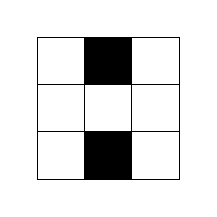
\begin{tikzpicture}
	\matrix [minimum width=0.6cm ,minimum height=0.6cm,row sep=-\pgflinewidth,column sep=-\pgflinewidth ]
	{
	\node [rectangle,draw] {}; & \node[rectangle,draw,fill=black]{}; & \node[rectangle,draw] {}; \\
	\node[rectangle,draw] {}; & \node[rectangle,draw] {$\blacklozenge$}; & \node[rectangle,draw] {}; \\
	\node[rectangle,draw] {}; & \node[rectangle,draw,fill=black]{}; & \node[rectangle,draw] {}; \\
	};
	\end{tikzpicture}
	\begin{tikzpicture}
	\matrix [minimum width=0.6cm ,minimum height=0.6cm,row sep=-\pgflinewidth,column sep=-\pgflinewidth ]
	{
	\node [rectangle,draw] {}; & \node[rectangle,draw] {$\blacklozenge$}; & \node[rectangle,draw] {};  \\
	};

	\end{tikzpicture}
	\end{center}
	\label{ej3_testcase5}
	\caption{Ejemplos de grilla sin solución}
\end{figure}


\subsubsection{Medición empírica de la performance}

A fin de verificar la cota teórica empíricamente, se realizaron múltiples
pruebas sobre grillas con todas sus celdas libres. En la \fig{fig:ej3_test_teo}
podemos observar como, en promedio, las mediciones tomadas para grillas con todas sus celdas
libre está por debajo de la cota teórica. Además se realizaron mediciones
sobre grillas cuadradas con diferentes porcentajes de paredes y 7\% de celdas
conteniendo reliquias, las misma distribuidas al azar. La \fig{fig:ej3_test_random}
muestra que los tiempos obtenidos son siempre menores a los obtenidos para grillas
con todas sus celdas libres.

%\begin{figure}[H]
%   \begin{center}
%   \includegraphics[width=1.4\textwidth,angle=90]{img/ejercicio3.png}
%   \caption{\textbf{Muestreo del Ejercicio 3}}
%   \label{fig:ej3}
%   \end{center}
%\end{figure}


\begin{figure}[H]
   \begin{center}
   \includegraphics[width=1.4\textwidth,angle=90]{img/grafico_ej3_teorica_vs_worst.pdf}
   \caption{\textbf{Muestreo del Ejercicio 3}}
   \label{fig:ej3_test_teo}
   \end{center}
\end{figure}


\begin{figure}[H]
   \begin{center}
   \includegraphics[width=1.4\textwidth,angle=90]{img/grafico_ej3_worst_vs_random_ej3.pdf}
   \caption{\textbf{Muestreo del Ejercicio 3 - Peor caso contra Casos aleatorios}}
   \label{fig:ej3_test_random}
   \end{center}
\end{figure}


% -----------------------------------------------
\end{document}
